\chapter{Results}

\section{Speed}

\subsection{LPFilter's Speed to Filtering Strength}

\begin{table}[htbp]
	\centering
	\begin{tabularx}{\textwidth}{|X|X|X|}
		\hline
		\textbf{Cut Off Frequency Hz} & \textbf{SMA processing time (ms)} & \textbf{EMA processing time (ms)} \\ \hline
		\textbf{20} & 2788 & 947 \\ \hline
		\textbf{500} & 11980 & 972 \\ \hline
		\textbf{1000} & 26930 & 972 \\ \hline
	\end{tabularx}
	\caption{Processing Time Comparison}
\end{table}


\begin{figure}[!h]
	\begin{center}
		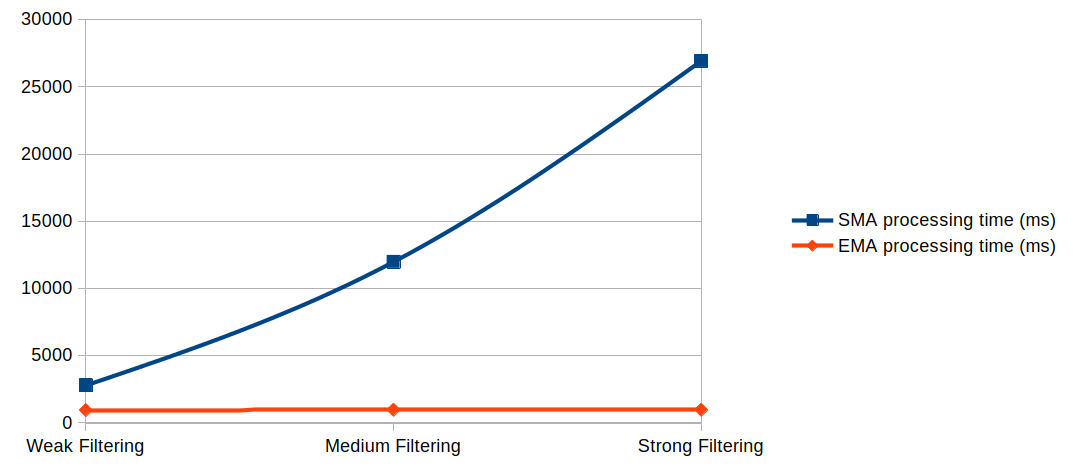
\includegraphics[width=15cm]{images/GraphSpeedtoFilteringStrength.png}
	\end{center}
	\caption{Processing speed of each filter as their cut off frequency decreases}
\end{figure}

\subsection{LPFilter's Speed to Data Length}

\begin{figure}[!h]
	\begin{center}
		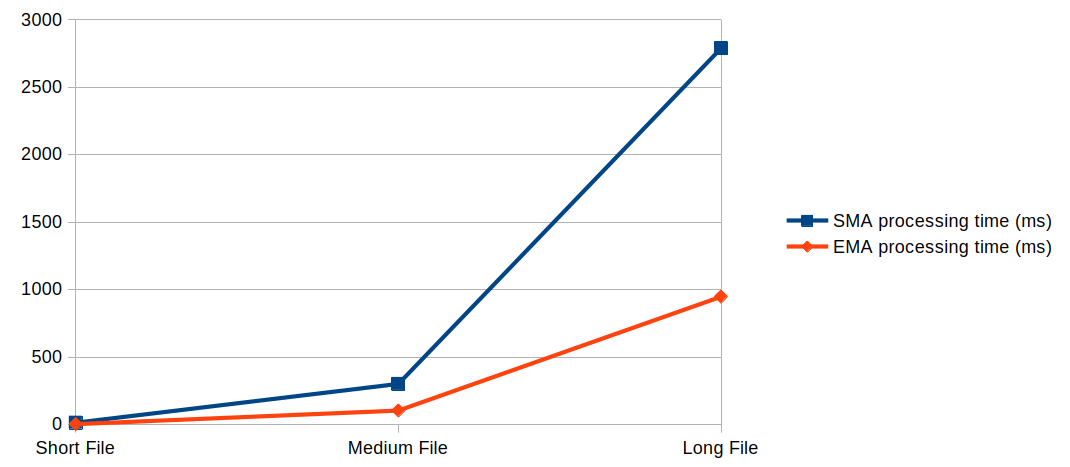
\includegraphics[width=15cm]{images/GraphSpeedtoLength.png}
	\end{center}
	\caption{Processing speed of each filters as the length of the data increases}
\end{figure}

\begin{table}[!h]
	\centering
	\begin{tabularx}{\textwidth}{|X|X|X|X|}
		\hline
		\textbf{File} & \textbf{Characters} & \textbf{SMA processing time (ms)} & \textbf{EMA processing time (ms)} \\ \hline
		\textbf{Short File} & \textbf{13} & 14 & 3 \\ \hline
		\textbf{Medium File} & \textbf{641} & 301 & 104 \\ \hline
		\textbf{Long File} & \textbf{6307} & 2788 & 947 \\ \hline
	\end{tabularx}
	\caption{Processing Time Comparison}
\end{table}

\subsection{LPFilter's Efficiency}

\begin{table}[!h]
	\centering
	\begin{tabularx}{\textwidth}{|X|X|X|X|}
		\hline
		\textbf{File} & \textbf{Characters} & \textbf{SMA processing time (ms)} & \textbf{EMA processing time (ms)} \\ \hline
		\textbf{Short File} & \textbf{13} & 14 & 3 \\ \hline
		\textbf{Medium File} & \textbf{641} & 301 & 104 \\ \hline
		\textbf{Long File} & \textbf{6307} & 2788 & 947 \\ \hline
	\end{tabularx}
	\caption{Processing Time Comparison}
\end{table}

\newpage

\subsection{LPFilter's Output}

\subsubsection{Filters Frequency Response and efficiency}

\begin{figure}[!h]
	\begin{center}
		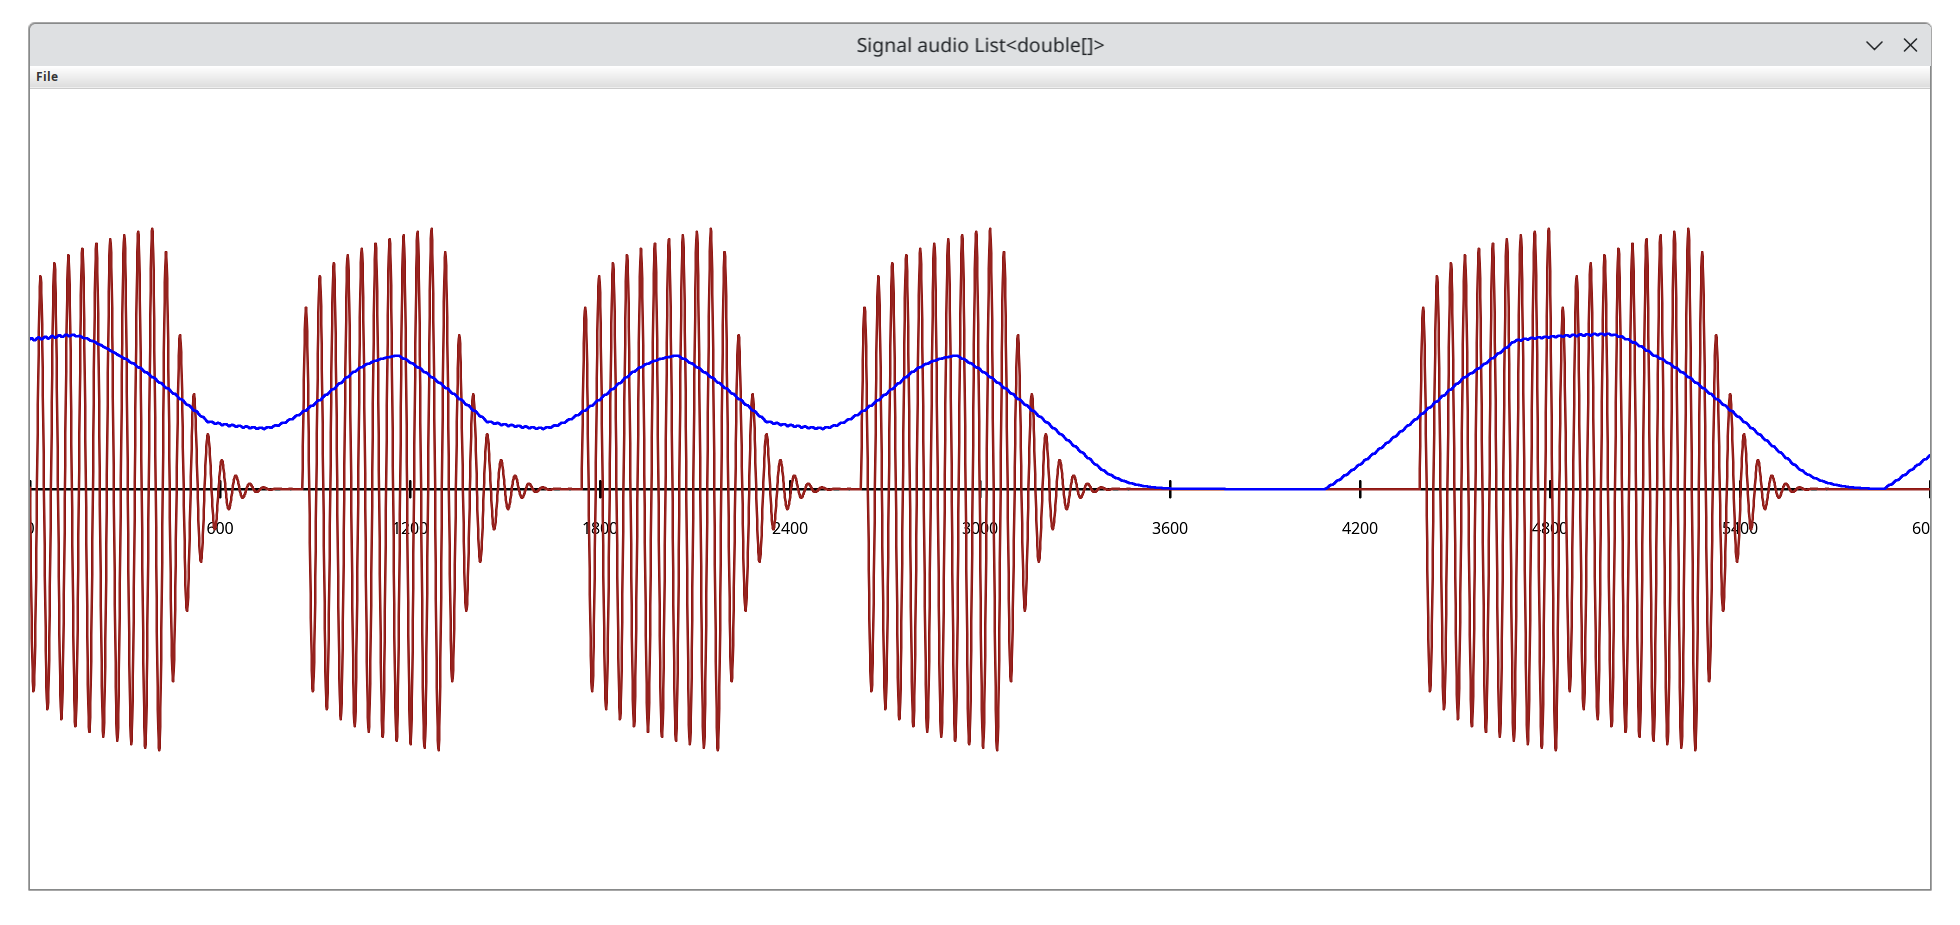
\includegraphics[width=15cm]{images/LP1600.png}
	\end{center}
	\caption{\textbf{SMA} Filter output in blue for a cut off frequency of \textbf{20Hz}}
\end{figure}

\begin{figure}[!h]
	\begin{center}
		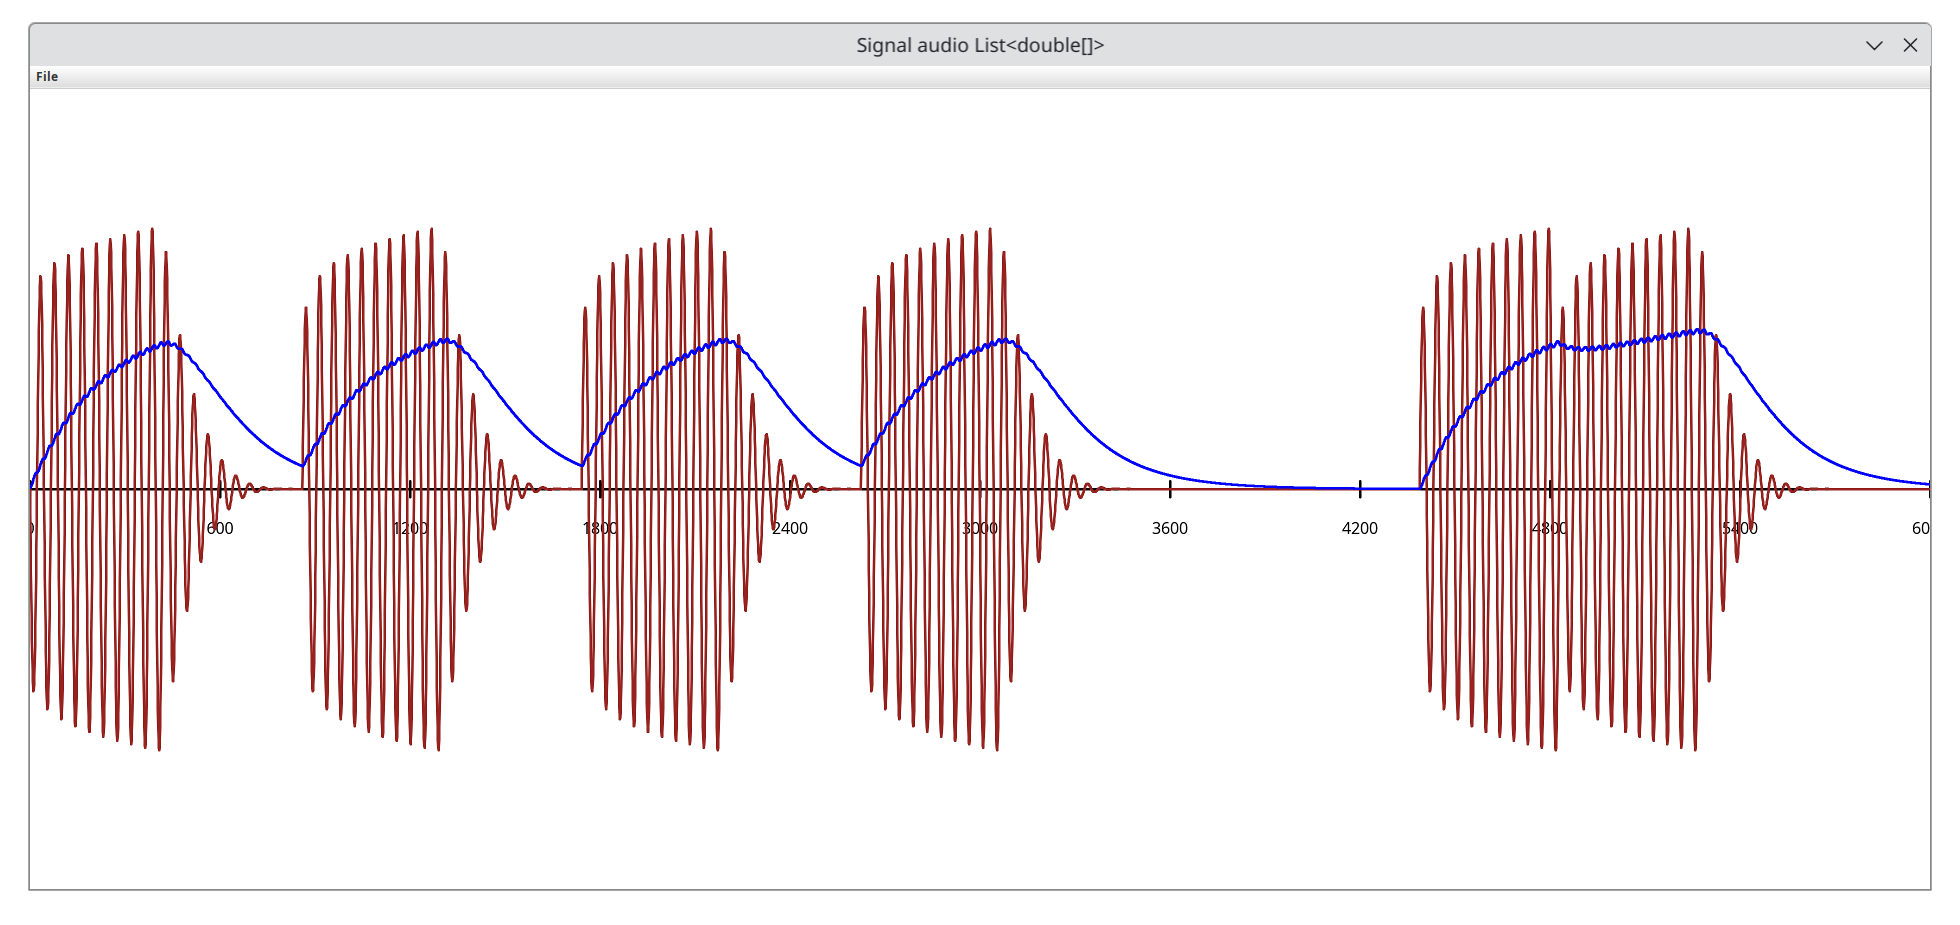
\includegraphics[width=15cm]{images/LP240.png}
	\end{center}
	\caption{\textbf{EMA} Filter output in blue for a cut off frequency of \textbf{20Hz}}
\end{figure}

\begin{figure}[!h]
	\begin{center}
		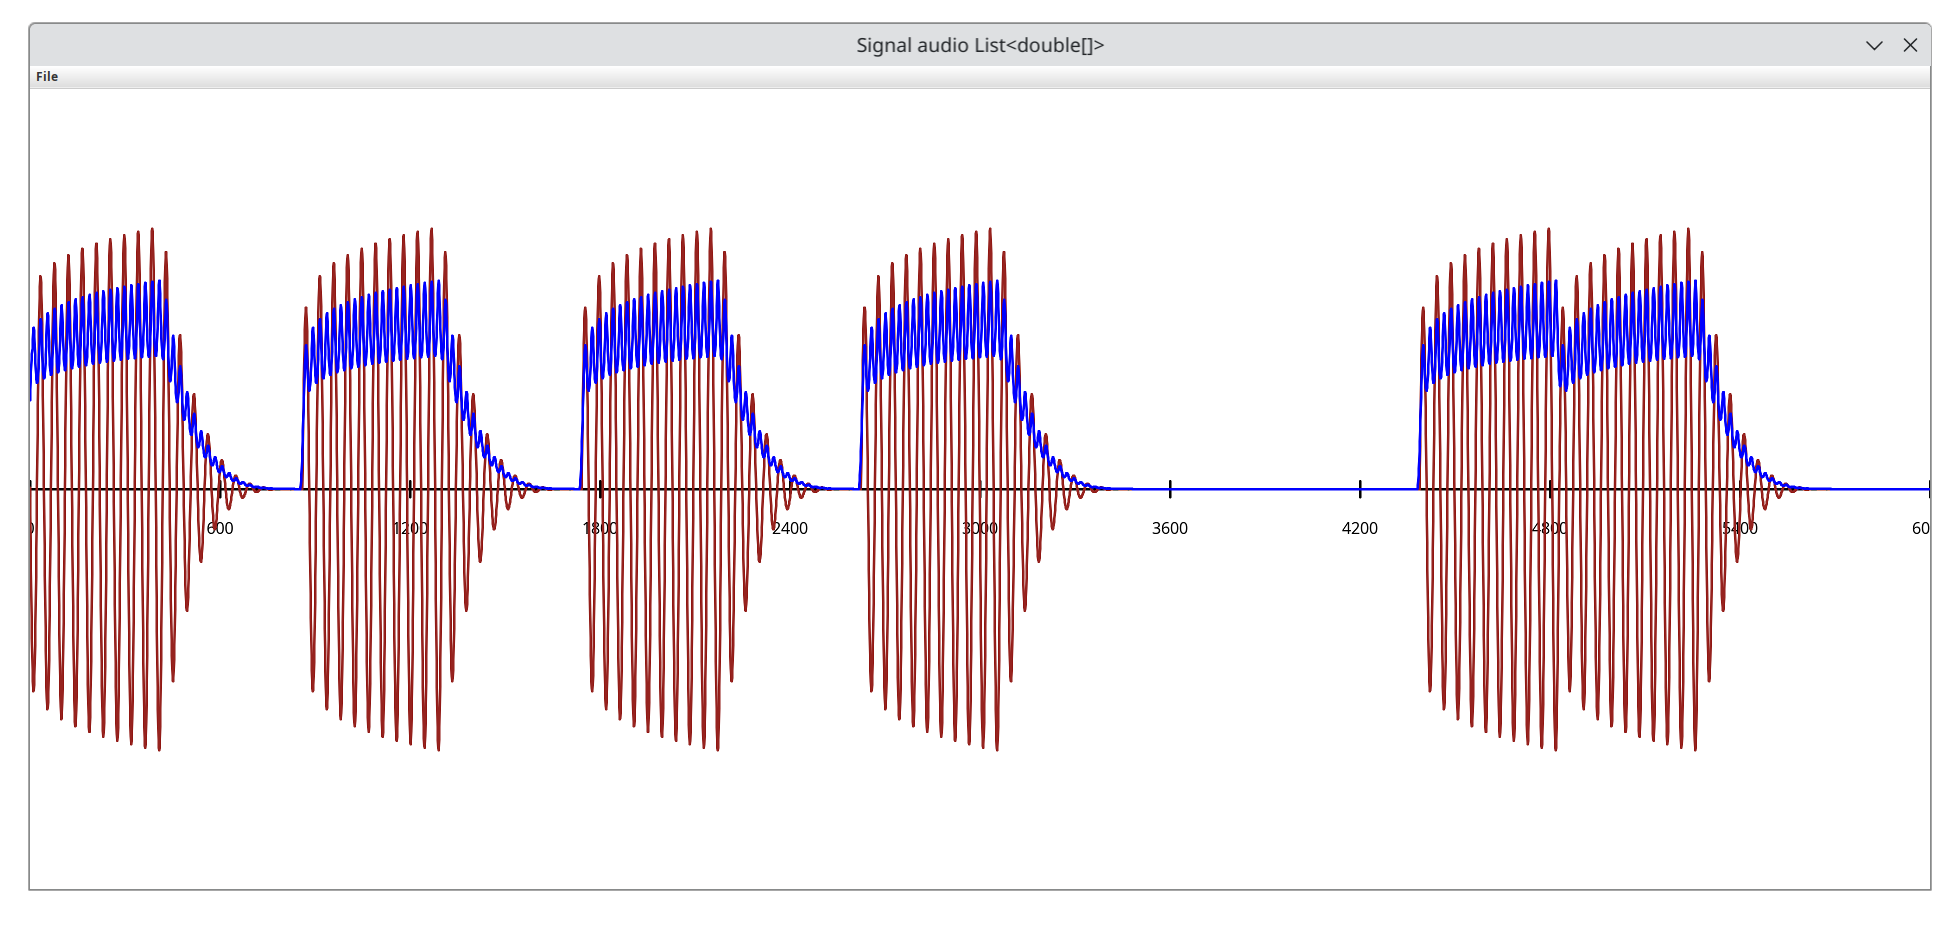
\includegraphics[width=15cm]{images/LP116.png}
	\end{center}
	\caption{\textbf{SMA} Filter output in blue for a cut off frequency of \textbf{1kHz}}
\end{figure}

\begin{figure}[!h]
	\begin{center}
		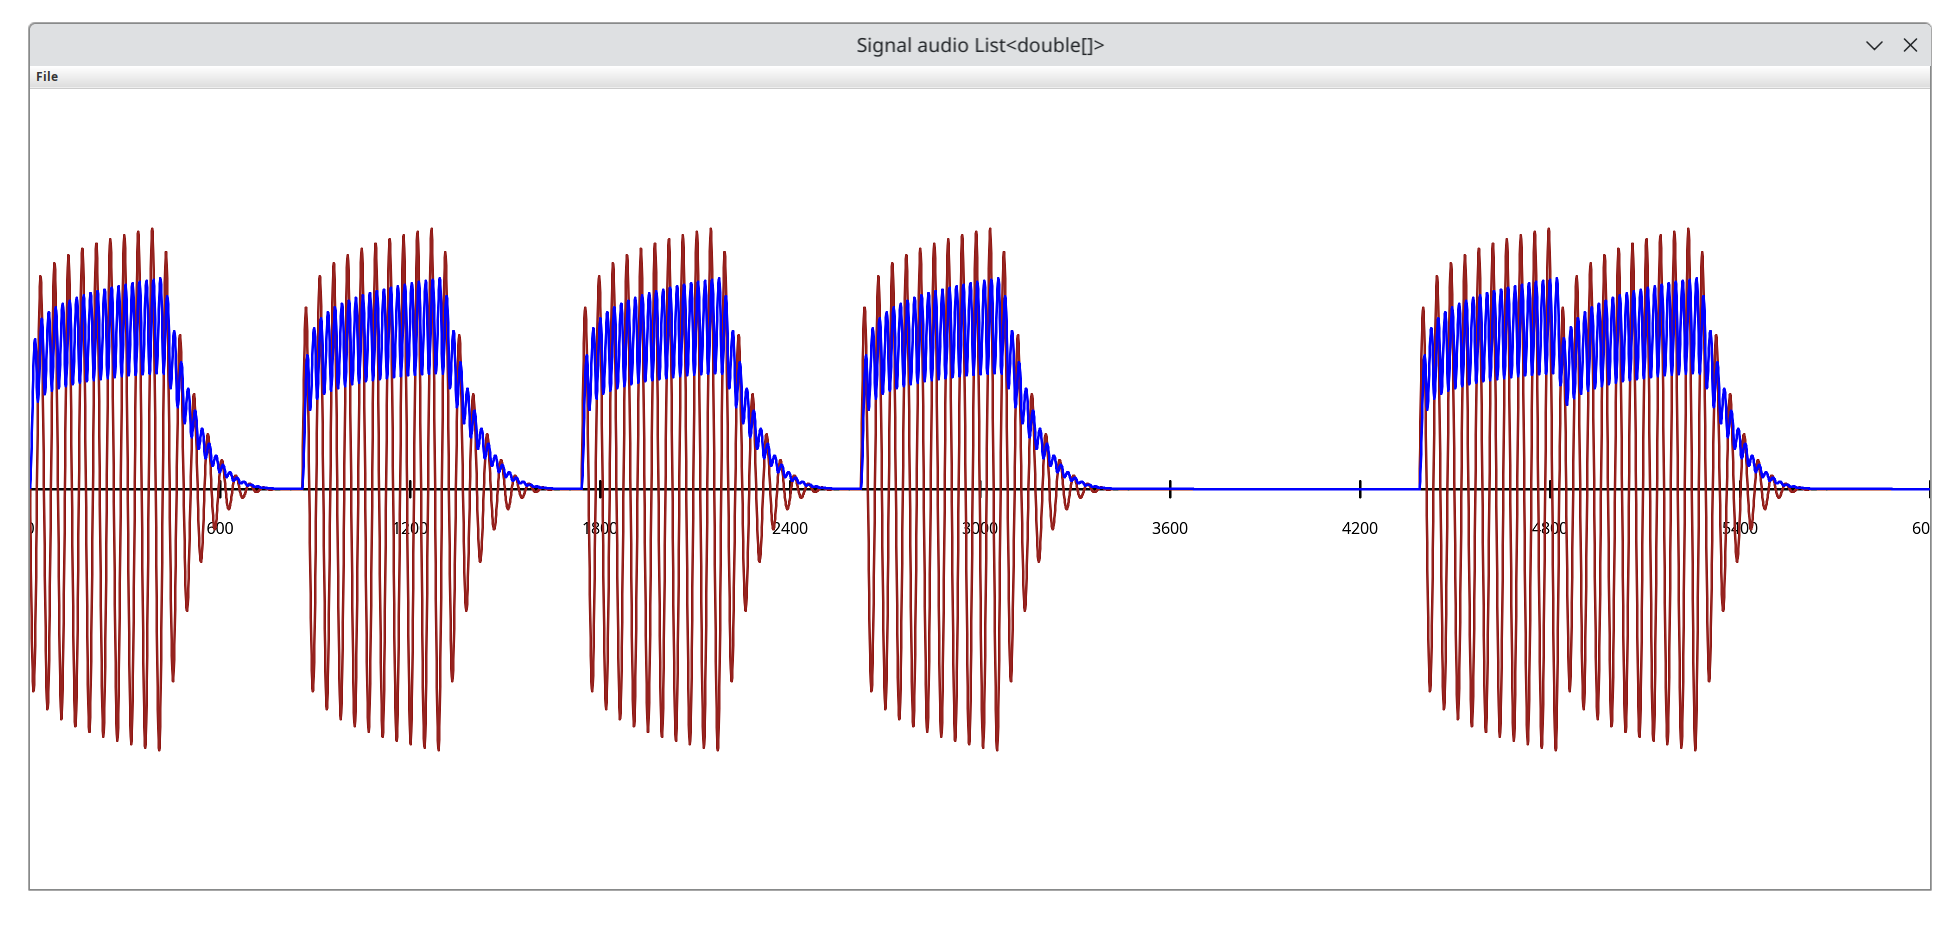
\includegraphics[width=15cm]{images/LP21000.png}
	\end{center}
	\caption{\textbf{EMA} Filter output in blue for a cut off frequency of \textbf{1kHz}}
\end{figure}

\begin{figure}[!h]
	\begin{center}
		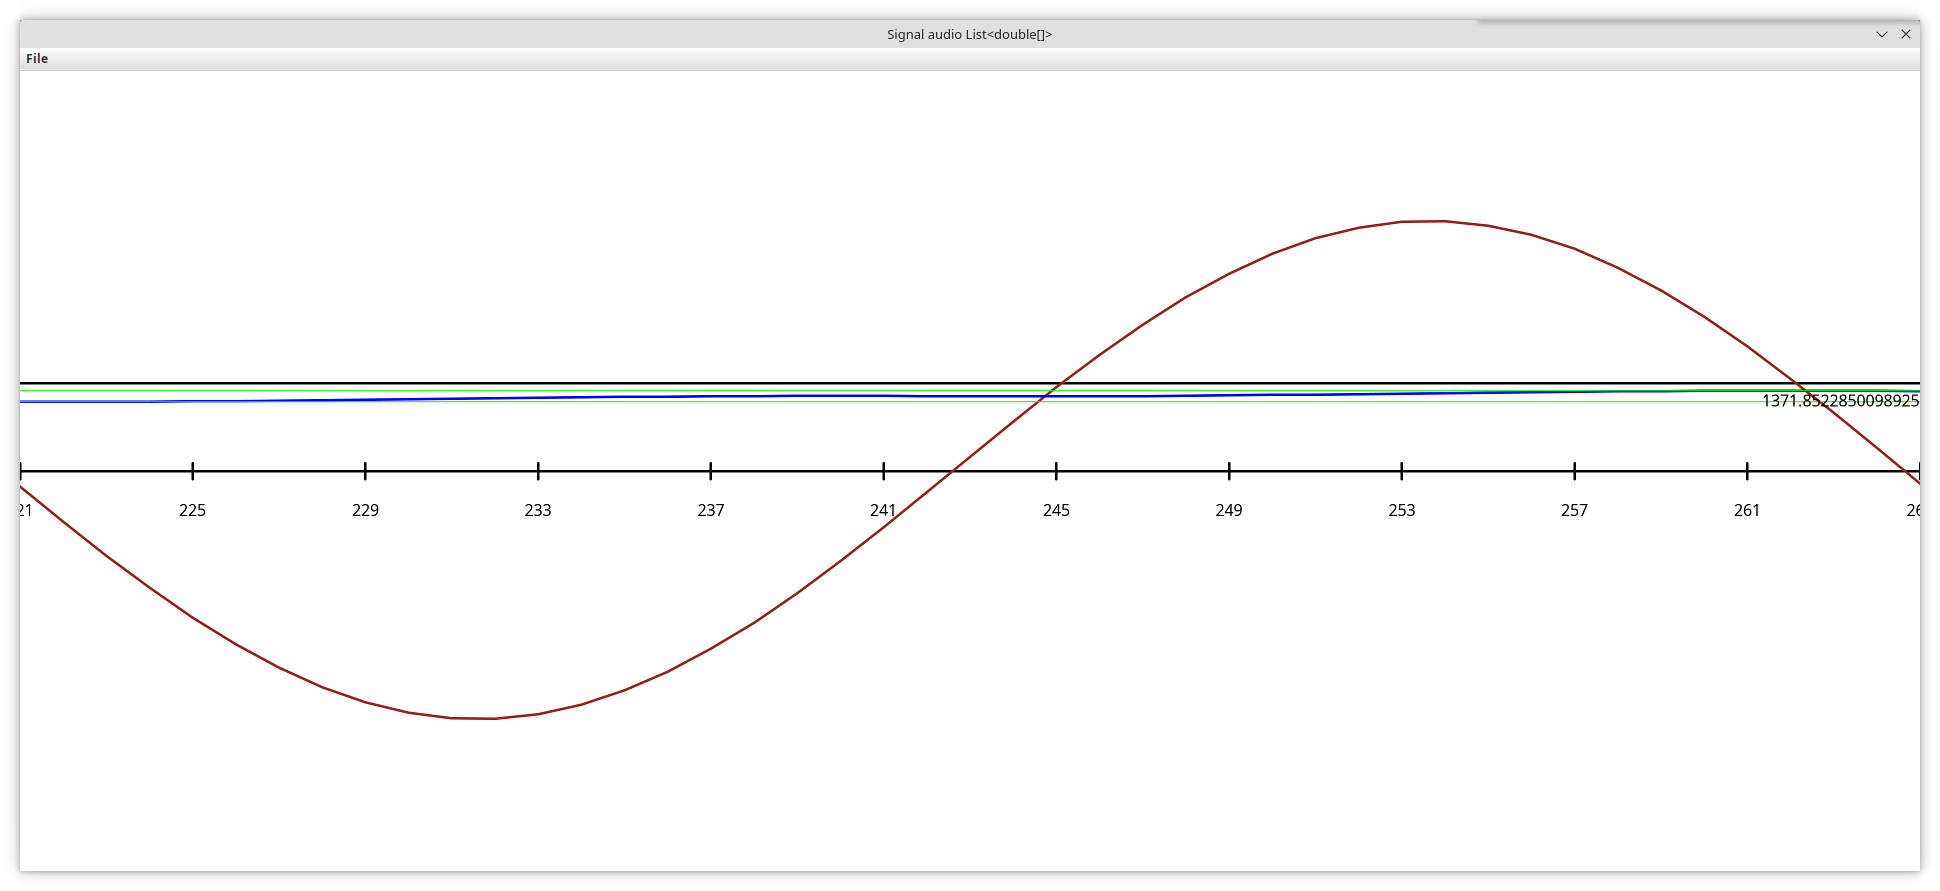
\includegraphics[width=15cm]{images/EMA20d1371.png}
	\end{center}
	\caption{\textbf{EMA} Delta of the signal amplitude for a cut off frequency value of 20Hz : 1371}
\end{figure}

\begin{figure}[!h]
	\begin{center}
		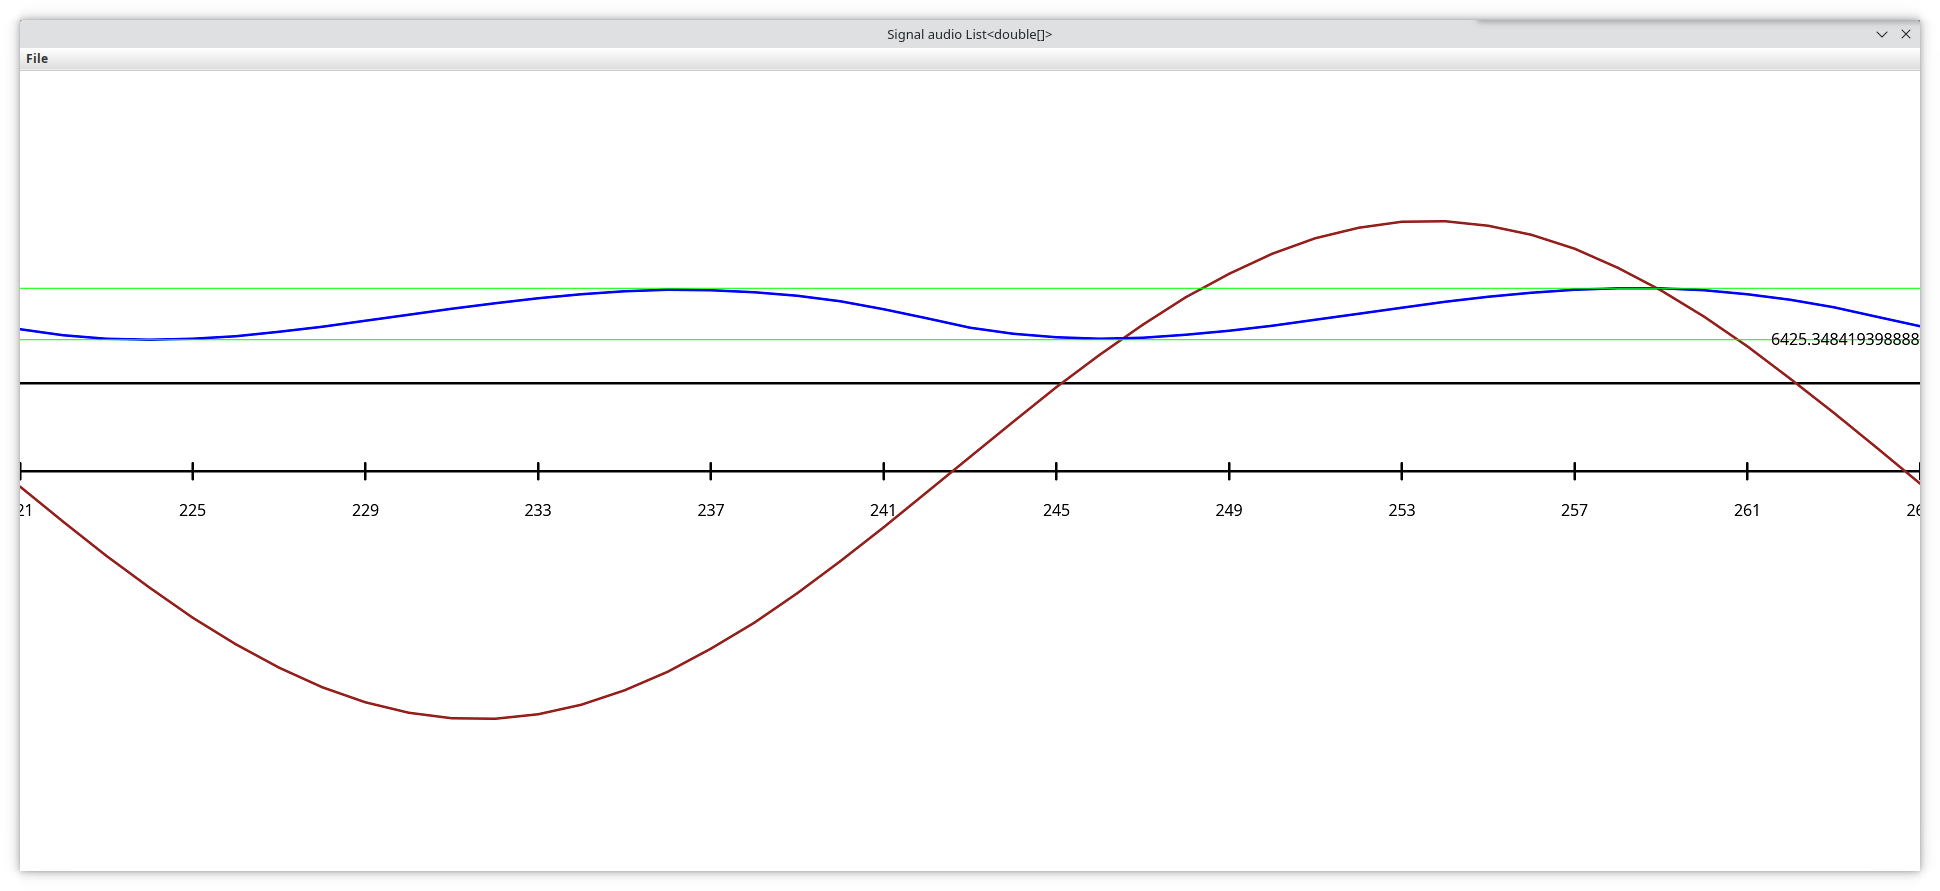
\includegraphics[width=15cm]{images/EMA500d6425.png}
	\end{center}
	\caption{\textbf{EMA} Delta of the signal amplitude for a cut off frequency value of 500Hz : 6425}
\end{figure}

\begin{figure}[!h]
	\begin{center}
		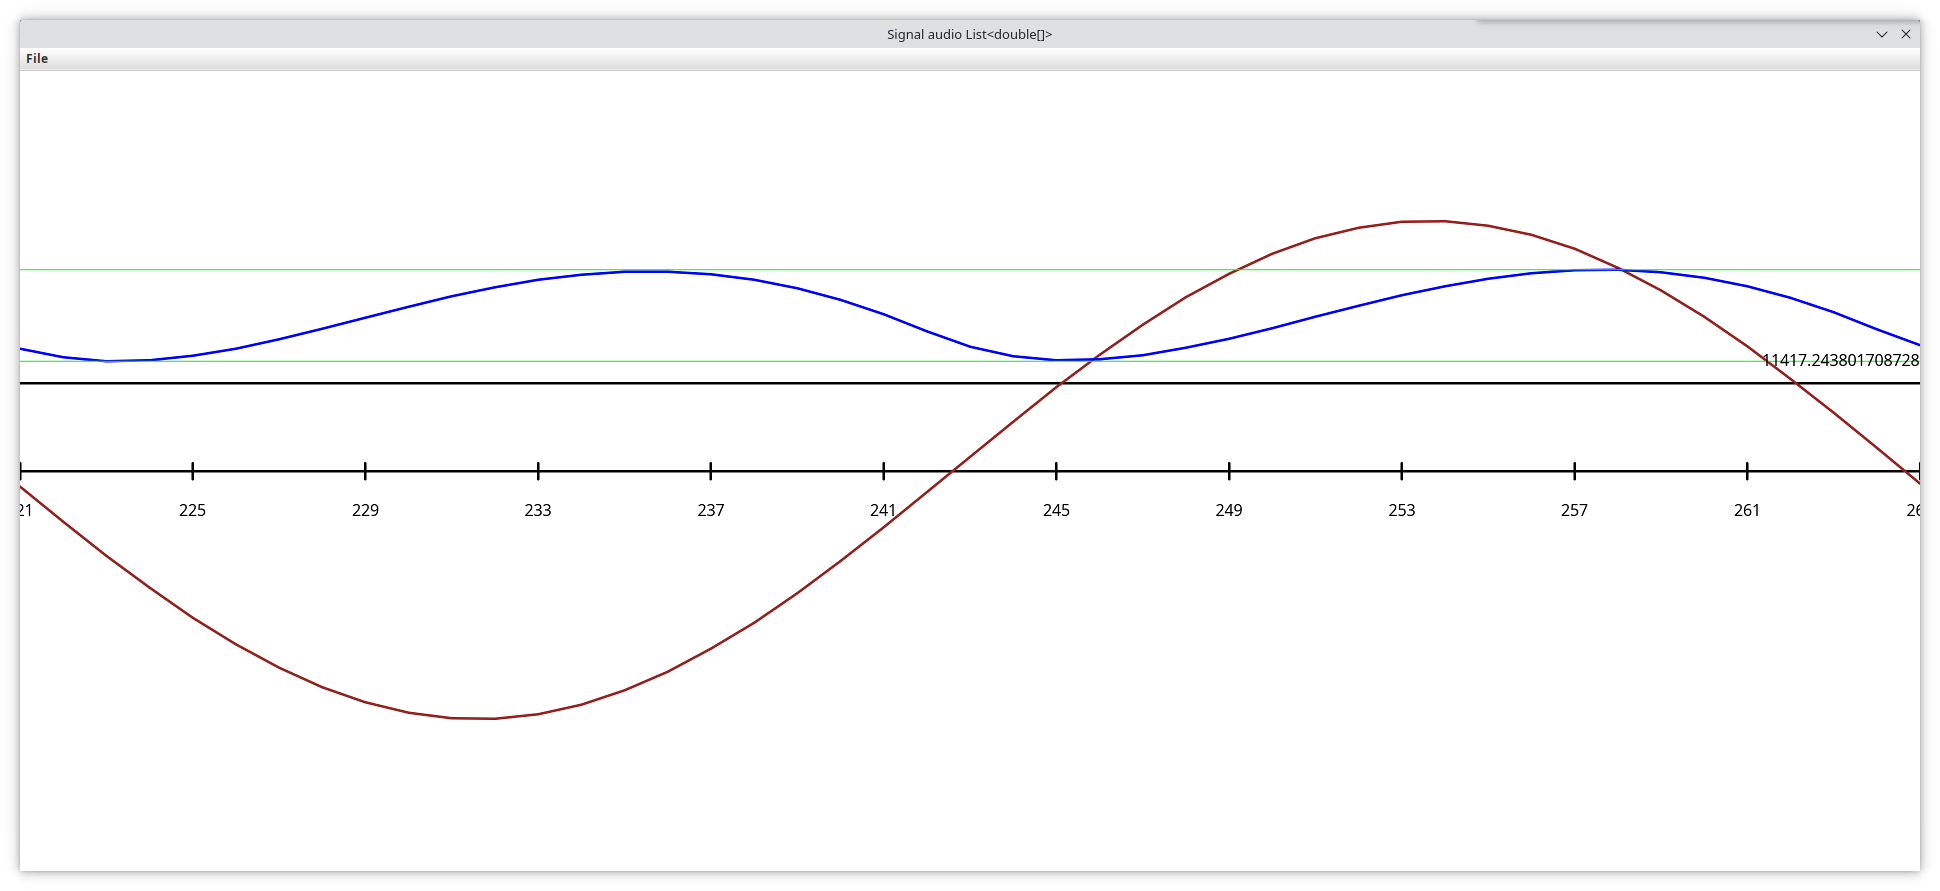
\includegraphics[width=15cm]{images/EMA1000d11417.png}
	\end{center}
	\caption{\textbf{EMA} Delta of the signal amplitude for a cut off frequency value of 1000Hz : 11417}
\end{figure}




